\documentclass[12pt,a4paper,final]{scrbook}
\usepackage[utf8]{inputenc}
\usepackage[ngerman]{babel}

\usepackage{graphicx}
\usepackage{subcaption}

\begin{document}
\chapter{Einführung}

Abbildung \ref{fig:Nikolaushaus} zeigt zwei Häuser. 
Abbildung \ref{fig:NikolaushausA} zeigt das aufrechte Haus vom Nikolaus und Abbildung \ref{fig:NikolaushausB} zeigt das um 90\textdegree~im Uhrzeigersinn gedrehte Haus vom Nikolaus. 

\begin{figure}[h!tb]
	\begin{subfigure}[b]{.49\textwidth} 
		\centering
		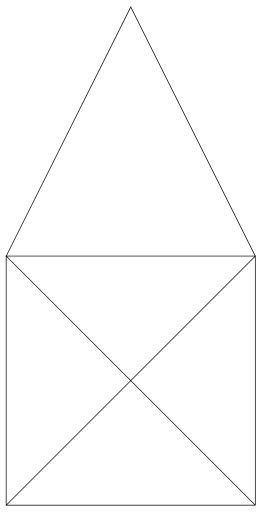
\includegraphics[width=2.5cm]{house.png}
		\caption{Das aufrechte Haus vom Nikolaus}
		\label{fig:NikolaushausA}
	\end{subfigure}
	\hfil
	\begin{subfigure}[b]{.49\textwidth}
		\centering
		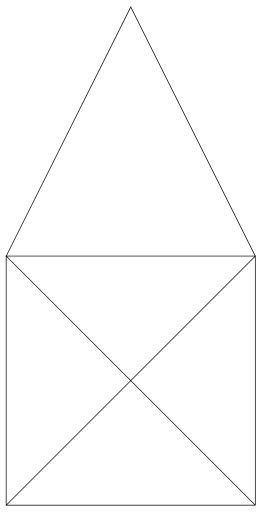
\includegraphics[width=2.5cm,angle=270]{house.png}
		\caption{Das Haus vom Nikolaus um 90\textdegree~im Uhrzeigersinn gedreht} 
		\label{fig:NikolaushausB}
	\end{subfigure}
\caption{Häuser vom Nikolaus}
\label{fig:Nikolaushaus}
\end{figure} 

\end{document}